% Options for packages loaded elsewhere
\PassOptionsToPackage{unicode}{hyperref}
\PassOptionsToPackage{hyphens}{url}
\PassOptionsToPackage{dvipsnames,svgnames,x11names}{xcolor}
%
\documentclass[
  12pt]{article}

\usepackage{amsmath,amssymb}
\usepackage{iftex}
\ifPDFTeX
  \usepackage[T1]{fontenc}
  \usepackage[utf8]{inputenc}
  \usepackage{textcomp} % provide euro and other symbols
\else % if luatex or xetex
  \usepackage{unicode-math}
  \defaultfontfeatures{Scale=MatchLowercase}
  \defaultfontfeatures[\rmfamily]{Ligatures=TeX,Scale=1}
\fi
\usepackage{lmodern}
\ifPDFTeX\else  
    % xetex/luatex font selection
\fi
% Use upquote if available, for straight quotes in verbatim environments
\IfFileExists{upquote.sty}{\usepackage{upquote}}{}
\IfFileExists{microtype.sty}{% use microtype if available
  \usepackage[]{microtype}
  \UseMicrotypeSet[protrusion]{basicmath} % disable protrusion for tt fonts
}{}
\makeatletter
\@ifundefined{KOMAClassName}{% if non-KOMA class
  \IfFileExists{parskip.sty}{%
    \usepackage{parskip}
  }{% else
    \setlength{\parindent}{0pt}
    \setlength{\parskip}{6pt plus 2pt minus 1pt}}
}{% if KOMA class
  \KOMAoptions{parskip=half}}
\makeatother
\usepackage{xcolor}
\setlength{\emergencystretch}{3em} % prevent overfull lines
\setcounter{secnumdepth}{5}
% Make \paragraph and \subparagraph free-standing
\makeatletter
\ifx\paragraph\undefined\else
  \let\oldparagraph\paragraph
  \renewcommand{\paragraph}{
    \@ifstar
      \xxxParagraphStar
      \xxxParagraphNoStar
  }
  \newcommand{\xxxParagraphStar}[1]{\oldparagraph*{#1}\mbox{}}
  \newcommand{\xxxParagraphNoStar}[1]{\oldparagraph{#1}\mbox{}}
\fi
\ifx\subparagraph\undefined\else
  \let\oldsubparagraph\subparagraph
  \renewcommand{\subparagraph}{
    \@ifstar
      \xxxSubParagraphStar
      \xxxSubParagraphNoStar
  }
  \newcommand{\xxxSubParagraphStar}[1]{\oldsubparagraph*{#1}\mbox{}}
  \newcommand{\xxxSubParagraphNoStar}[1]{\oldsubparagraph{#1}\mbox{}}
\fi
\makeatother


\providecommand{\tightlist}{%
  \setlength{\itemsep}{0pt}\setlength{\parskip}{0pt}}\usepackage{longtable,booktabs,array}
\usepackage{calc} % for calculating minipage widths
% Correct order of tables after \paragraph or \subparagraph
\usepackage{etoolbox}
\makeatletter
\patchcmd\longtable{\par}{\if@noskipsec\mbox{}\fi\par}{}{}
\makeatother
% Allow footnotes in longtable head/foot
\IfFileExists{footnotehyper.sty}{\usepackage{footnotehyper}}{\usepackage{footnote}}
\makesavenoteenv{longtable}
\usepackage{graphicx}
\makeatletter
\def\maxwidth{\ifdim\Gin@nat@width>\linewidth\linewidth\else\Gin@nat@width\fi}
\def\maxheight{\ifdim\Gin@nat@height>\textheight\textheight\else\Gin@nat@height\fi}
\makeatother
% Scale images if necessary, so that they will not overflow the page
% margins by default, and it is still possible to overwrite the defaults
% using explicit options in \includegraphics[width, height, ...]{}
\setkeys{Gin}{width=\maxwidth,height=\maxheight,keepaspectratio}
% Set default figure placement to htbp
\makeatletter
\def\fps@figure{htbp}
\makeatother

\addtolength{\oddsidemargin}{-.5in}%
\addtolength{\evensidemargin}{-1in}%
\addtolength{\textwidth}{1in}%
\addtolength{\textheight}{1.7in}%
\addtolength{\topmargin}{-1in}%
\usepackage{booktabs}
\usepackage{longtable}
\usepackage{array}
\usepackage{multirow}
\usepackage{wrapfig}
\usepackage{float}
\usepackage{colortbl}
\usepackage{pdflscape}
\usepackage{tabu}
\usepackage{threeparttable}
\usepackage{threeparttablex}
\usepackage[normalem]{ulem}
\usepackage{makecell}
\usepackage{xcolor}
\makeatletter
\@ifpackageloaded{caption}{}{\usepackage{caption}}
\AtBeginDocument{%
\ifdefined\contentsname
  \renewcommand*\contentsname{Table of contents}
\else
  \newcommand\contentsname{Table of contents}
\fi
\ifdefined\listfigurename
  \renewcommand*\listfigurename{List of Figures}
\else
  \newcommand\listfigurename{List of Figures}
\fi
\ifdefined\listtablename
  \renewcommand*\listtablename{List of Tables}
\else
  \newcommand\listtablename{List of Tables}
\fi
\ifdefined\figurename
  \renewcommand*\figurename{Figure}
\else
  \newcommand\figurename{Figure}
\fi
\ifdefined\tablename
  \renewcommand*\tablename{Table}
\else
  \newcommand\tablename{Table}
\fi
}
\@ifpackageloaded{float}{}{\usepackage{float}}
\floatstyle{ruled}
\@ifundefined{c@chapter}{\newfloat{codelisting}{h}{lop}}{\newfloat{codelisting}{h}{lop}[chapter]}
\floatname{codelisting}{Listing}
\newcommand*\listoflistings{\listof{codelisting}{List of Listings}}
\makeatother
\makeatletter
\makeatother
\makeatletter
\@ifpackageloaded{caption}{}{\usepackage{caption}}
\@ifpackageloaded{subcaption}{}{\usepackage{subcaption}}
\makeatother
\ifLuaTeX
  \usepackage{selnolig}  % disable illegal ligatures
\fi
\usepackage[]{natbib}
\bibliographystyle{agsm}
\usepackage{bookmark}

\IfFileExists{xurl.sty}{\usepackage{xurl}}{} % add URL line breaks if available
\urlstyle{same} % disable monospaced font for URLs
\hypersetup{
  pdftitle={Some simple approaches to improve the Welch- Satterthwaite approximation},
  pdfauthor={Carlos Alberto Cardozo Delgado; Luis Francisco Gómez López},
  pdfkeywords={Asymmetric distributions, Unbiased estimation, Consistent
estimation, Monte Carlo simulation},
  colorlinks=true,
  linkcolor={blue},
  filecolor={Maroon},
  citecolor={Blue},
  urlcolor={Blue},
  pdfcreator={LaTeX via pandoc}}


\begin{document}


\def\spacingset#1{\renewcommand{\baselinestretch}%
{#1}\small\normalsize} \spacingset{1}


%%%%%%%%%%%%%%%%%%%%%%%%%%%%%%%%%%%%%%%%%%%%%%%%%%%%%%%%%%%%%%%%%%%%%%%%%%%%%%

\date{June 26, 2024}
\title{\bf Some simple approaches to improve the Welch- Satterthwaite
approximation}
\author{
Carlos Alberto Cardozo Delgado\thanks{The authors gratefully acknowledge
\emph{please remember to list all relevant funding sources in the
non-anonymized (unblinded) version}.}\\
Departamento de Matemáticas, Pontificia Universidad Javeriana\\
and\\Luis Francisco Gómez López\\
Administración de Empresas, Universidad Militar Nueva Granada\\
}
\maketitle

\bigskip
\bigskip
\begin{abstract}
In this work we propose three simple ways to improve the classical
Welch-Satterthwaite (WS) approximation to the effective degree of
freedom of a non-negative linear combination of \(\chi^2\)
distributions. The WS option is typically used in design of experiments
and metrology. However, it has been pointing out in many references the
multiple limitations of the inferences based on the WS approximation.
Three novel estimators of the effective degree of freedom of a
non-negative linear combination of \(\chi^2\) distributions are given.
We also study some theoretical properties of the proposed estimators.
Additionally, through several Monte Carlo simulations, we assess the
bias, variance, and mean square error of the proposed estimators under
(very) small and moderate sample sizes. The proposed estimators have a
much better performance than the WS proposal and his implications.
Finally, two applications are presented in which the proposed estimators
help to improve the performance of some interval estimation and
hypothesis testing procedures.
\end{abstract}

\noindent%
{\it Keywords:} Asymmetric distributions, Unbiased
estimation, Consistent estimation, Monte Carlo simulation
\vfill

\newpage
\spacingset{1.9} % DON'T change the spacing!

\section{Introduction}\label{sec-intro}

\section{Critical aspects of the WS
approach}\label{critical-aspects-of-the-ws-approach}

\citet{lloyd_2-sample_2013} conducted three numerical experiments
highlighting potential limitations of the two-sample t-test when using
the Welch-Satterthwaite (WS) approximation. Notably, in their first
experiment, \citet{lloyd_2-sample_2013} assumed that the ratio of
population variances was known. However, in practice, this information
is rarely available. Therefore, we will replicate this simulation
without assuming a known variance ratio, providing a more realistic
assessment of the two-sample t-test's performance under the WS
approximation.

We now outline the initial simulation plan associated with the
two-sample t-test statistic,
\(T = \frac{\overline{X} - \overline{Y} - (\mu_1 - \mu_2)}{\sqrt{\frac{\widehat{\sigma}^2_1}{n_1} + \frac{\widehat{\sigma}^2_2}{n_2}}}\).
Let
\(X_1, X_2, \ldots, X_{n_1} \overset{\text{iid}}{\sim} \mathcal{N}(\mu_1, \sigma_1^2)\)
and
\(Y_1, Y_2, \ldots, Y_{n_2} \overset{\text{iid}}{\sim} \mathcal{N}(\mu_2, \sigma_2^2)\)
where \(\mathbf{X} = (X_1, X_2, \ldots, X_{n_1})\) and
\(\mathbf{Y} = (Y_1, Y_2, \ldots, Y_{n_2})\) are 2 independent random
vectors. We assume the following parameters:

\begin{itemize}
\tightlist
\item
  \(\mu_1 = 1\) and \(\mu_2 = 2\).
\item
  \(\sigma^2_1 = 1\) and varying variance ratios,
  \(\frac{\sigma^2_2}{\sigma^2_1} \equiv \rho = 2, 4, 6, 8, 10, 12\).
\item
  \(n_1\) takes values \(n_1 = 2, 3, \ldots, 14\), with sample size
  ratios, \(\frac{n_2}{n_1} \equiv k = 1, 2, 4\).
\end{itemize}

For each combination of \((\rho, n_1, k)\), we construct the sampling
distribution of the two-sample t-test statistic based on \(R = 10000\)
replications. In contrast to \citet{lloyd_2-sample_2013}, we do not
pre-calculate and fix the degrees of freedom, \(\nu\), using the WS
approach. Instead, for each replication, we estimate the degrees of
freedom, denoted by \(\widehat{\nu}\), using the WS approach (see
Section~\ref{sec-df-ws} for details). Next, we determine the lower and
upper critical values, \(t_{\alpha,\widehat{\nu}}\) and
\(t_{1-\alpha,\widehat{\nu}}\), respectively for \(\alpha = 0.05, 0.10\)
to calculate the corresponding type I error rates based on the WS
approach as\footnote{The index \(j\) takes on values from \(1\) to
  \(468\) because \(\rho\) takes \(6\), \(n_1\) \(13\), \(k\) \(3\) and
  \(\alpha\) \(2\) values. Therefore \(\widehat{\alpha}_j\) can take
  \(468\) values.}:

\begin{equation}\phantomsection\label{eq-type-I-error-rates}{\widehat{\alpha}_j = F_{T}\left(t_{\alpha,\widehat{\nu}}\right) + \left(1 - F_{T}\left(t_{1-\alpha,\widehat{\nu}}\right)\right) \text{ for } j = 1, 2, \ldots, 468}\end{equation}

Finally, to assess the accuracy of the estimated type I error rates, we
calculate the relative difference between each \(\widehat{\alpha}_j\)
and the corresponding true significance level \(\alpha\) and compare it
to a threshold of \(d=0.10\):

\begin{equation}\phantomsection\label{eq-pro-rel-alpha}{\frac{|\widehat{\alpha}_j - \alpha|}{\alpha} > d = 0.10}\end{equation}

where \(F_T\) represents the empirical cumulative distribution function
of the two-sample t-test statistic. Table~\ref{tbl-sim-pro-rel-alpha}
presents the results for the combination \((\rho, n_1, k, \alpha)\).
Figure~\ref{fig-sim-pro-rel-alpha} provides a visual representation of
these results.

\begingroup\fontsize{7}{9}\selectfont

\begin{longtable}[t]{rrrrrrrrrrrrrrrr}

\caption{\label{tbl-sim-pro-rel-alpha}Proportion of replicates where the
relative absolute difference between a nominal \(\alpha\) and the
\(\alpha\)-value given by WS approximation test is bigger than
\(d=0.10\) where \(\alpha = 0.1, 0.05\)}

\tabularnewline

\toprule
\multicolumn{3}{c}{ } & \multicolumn{13}{c}{$n_1$} \\
\cmidrule(l{3pt}r{3pt}){4-16}
$\alpha$ & $k$ & $\rho$ & 2 & 3 & 4 & 5 & 6 & 7 & 8 & 9 & 10 & 11 & 12 & 13 & 14\\
\midrule
\endfirsthead
\multicolumn{16}{@{}l}{\textit{(continued)}}\\
\toprule
$\alpha$ & $k$ & $\rho$ & 2 & 3 & 4 & 5 & 6 & 7 & 8 & 9 & 10 & 11 & 12 & 13 & 14\\
\midrule
\endhead

\endfoot
\bottomrule
\endlastfoot
 &  & 2 & 0.8167 & 0.7278 & 0.4823 & 0.4344 & 0.3454 & 0.3640 & 0.0996 & 0.1619 & 0.2307 & 0.0263 & 0.0355 & 0.0311 & 0.0327\\
\cmidrule{3-16}\nopagebreak
 &  & 4 & 0.8812 & 0.8185 & 0.7612 & 0.6718 & 0.4648 & 0.3742 & 0.4741 & 0.2804 & 0.1602 & 0.1177 & 0.7672 & 0.0224 & 0.0005\\
\cmidrule{3-16}\nopagebreak
 &  & 6 & 0.9374 & 0.8681 & 0.8057 & 0.7048 & 0.5605 & 0.4985 & 0.3278 & 0.2393 & 0.1502 & 0.1876 & 0.1355 & 0.0000 & 0.2764\\
\cmidrule{3-16}\nopagebreak
 &  & 8 & 0.9479 & 0.8708 & 0.8216 & 0.7498 & 0.5562 & 0.3923 & 0.3538 & 0.1622 & 0.0803 & 0.1163 & 0.1551 & 0.0718 & 0.0222\\
\cmidrule{3-16}\nopagebreak
 &  & 10 & 0.9483 & 0.8683 & 0.8089 & 0.5081 & 0.4541 & 0.2961 & 0.2114 & 0.1665 & 0.1182 & 0.0506 & 0.1046 & 0.1443 & 0.0277\\
\cmidrule{3-16}\nopagebreak
 & \multirow{-6}{*}{\raggedleft\arraybackslash 1} & 12 & 0.9507 & 0.8337 & 0.7890 & 0.7432 & 0.5647 & 0.1711 & 0.2139 & 0.1234 & 0.2052 & 0.0293 & 0.1535 & 0.0058 & 0.0008\\
\cmidrule{2-16}\nopagebreak
 &  & 2 & 0.6179 & 0.4658 & 0.3532 & 0.2058 & 0.2722 & 0.2404 & 0.0869 & 0.1195 & 0.0194 & 0.0432 & 0.0005 & 0.0212 & 0.0001\\
\cmidrule{3-16}\nopagebreak
 &  & 4 & 0.6605 & 0.4525 & 0.3374 & 0.0782 & 0.1883 & 0.0805 & 0.0357 & 0.0359 & 0.0594 & 0.0000 & 0.0025 & 0.0001 & 0.0000\\
\cmidrule{3-16}\nopagebreak
 &  & 6 & 0.6871 & 0.3774 & 0.2895 & 0.0864 & 0.1181 & 0.0022 & 0.0022 & 0.0105 & 0.0006 & 0.0007 & 0.0000 & 0.0000 & 0.0000\\
\cmidrule{3-16}\nopagebreak
 &  & 8 & 0.6079 & 0.4828 & 0.2353 & 0.0481 & 0.1129 & 0.0005 & 0.0002 & 0.0024 & 0.1255 & 0.0001 & 0.0000 & 0.0000 & 0.0000\\
\cmidrule{3-16}\nopagebreak
 &  & 10 & 0.6460 & 0.5698 & 0.3205 & 0.0747 & 0.3035 & 0.3759 & 0.0001 & 0.0206 & 0.0000 & 0.0000 & 0.0000 & 0.0000 & 0.0000\\
\cmidrule{3-16}\nopagebreak
 & \multirow{-6}{*}{\raggedleft\arraybackslash 2} & 12 & 0.6499 & 0.5901 & 0.5432 & 0.2027 & 0.0337 & 0.0234 & 0.0003 & 0.0005 & 0.0454 & 0.0002 & 0.0000 & 0.0000 & 0.0000\\
\cmidrule{2-16}\nopagebreak
 &  & 2 & 0.9635 & 0.9177 & 0.8081 & 0.6863 & 0.7018 & 0.4799 & 0.2746 & 0.4165 & 0.3697 & 0.3393 & 0.1927 & 0.2494 & 0.0572\\
\cmidrule{3-16}\nopagebreak
 &  & 4 & 0.9561 & 0.8365 & 0.7511 & 0.6326 & 0.4655 & 0.4090 & 0.4557 & 0.2695 & 0.2326 & 0.0184 & 0.4717 & 0.0155 & 0.6314\\
\cmidrule{3-16}\nopagebreak
 &  & 6 & 0.8965 & 0.3858 & 0.2982 & 0.5691 & 0.1231 & 0.0849 & 0.0924 & 0.0258 & 0.4758 & 0.1435 & 0.1359 & 0.0005 & 0.0001\\
\cmidrule{3-16}\nopagebreak
 &  & 8 & 0.3722 & 0.3178 & 0.3098 & 0.1777 & 0.0651 & 0.0425 & 0.0396 & 0.0565 & 0.0446 & 0.0000 & 0.0001 & 0.0025 & 0.0067\\
\cmidrule{3-16}\nopagebreak
 &  & 10 & 0.3818 & 0.2726 & 0.4143 & 0.1520 & 0.0618 & 0.0171 & 0.0480 & 0.1614 & 0.0077 & 0.0001 & 0.0001 & 0.0000 & 0.0002\\
\cmidrule{3-16}\nopagebreak
\multirow{-18}{*}[1\dimexpr\aboverulesep+\belowrulesep+\cmidrulewidth]{\raggedleft\arraybackslash 0.05} & \multirow{-6}{*}{\raggedleft\arraybackslash 4} & 12 & 0.3304 & 0.5526 & 0.2300 & 0.1283 & 0.0525 & 0.0298 & 0.0226 & 0.0015 & 0.0271 & 0.0321 & 0.0000 & 0.0000 & 0.0000\\
\cmidrule{1-16}\pagebreak[0]
 &  & 2 & 0.7805 & 0.5420 & 0.4423 & 0.2567 & 0.2412 & 0.1881 & 0.0066 & 0.0007 & 0.0100 & 0.0023 & 0.0000 & 0.0000 & 0.0000\\
\cmidrule{3-16}\nopagebreak
 &  & 4 & 0.8475 & 0.7629 & 0.6078 & 0.3310 & 0.2239 & 0.2092 & 0.1698 & 0.0000 & 0.0149 & 0.0000 & 0.3477 & 0.0000 & 0.0000\\
\cmidrule{3-16}\nopagebreak
 &  & 6 & 0.8932 & 0.7518 & 0.6312 & 0.4281 & 0.3514 & 0.1369 & 0.1128 & 0.0019 & 0.0018 & 0.0000 & 0.0800 & 0.0000 & 0.1081\\
\cmidrule{3-16}\nopagebreak
 &  & 8 & 0.9124 & 0.7944 & 0.6258 & 0.4558 & 0.2437 & 0.1706 & 0.0090 & 0.0034 & 0.0064 & 0.0000 & 0.0000 & 0.0000 & 0.0015\\
\cmidrule{3-16}\nopagebreak
 &  & 10 & 0.9266 & 0.7692 & 0.5972 & 0.2522 & 0.1116 & 0.1387 & 0.0279 & 0.0321 & 0.0113 & 0.0090 & 0.0042 & 0.0000 & 0.0052\\
\cmidrule{3-16}\nopagebreak
 & \multirow{-6}{*}{\raggedleft\arraybackslash 1} & 12 & 0.9180 & 0.7894 & 0.6412 & 0.4132 & 0.1348 & 0.1147 & 0.1178 & 0.0345 & 0.0732 & 0.0000 & 0.0017 & 0.0000 & 0.0033\\
\cmidrule{2-16}\nopagebreak
 &  & 2 & 0.6344 & 0.3654 & 0.2897 & 0.1178 & 0.1178 & 0.0651 & 0.0310 & 0.0195 & 0.0008 & 0.0095 & 0.0000 & 0.0020 & 0.0000\\
\cmidrule{3-16}\nopagebreak
 &  & 4 & 0.6267 & 0.3008 & 0.3186 & 0.0329 & 0.0423 & 0.0083 & 0.0036 & 0.0109 & 0.0022 & 0.0000 & 0.0000 & 0.0000 & 0.0000\\
\cmidrule{3-16}\nopagebreak
 &  & 6 & 0.5847 & 0.3843 & 0.0561 & 0.0139 & 0.0224 & 0.0001 & 0.0008 & 0.0002 & 0.0000 & 0.0000 & 0.0000 & 0.0000 & 0.0000\\
\cmidrule{3-16}\nopagebreak
 &  & 8 & 0.6022 & 0.3061 & 0.0440 & 0.0203 & 0.0018 & 0.0000 & 0.0000 & 0.0000 & 0.0001 & 0.0001 & 0.0000 & 0.0000 & 0.0000\\
\cmidrule{3-16}\nopagebreak
 &  & 10 & 0.5117 & 0.4837 & 0.1780 & 0.0017 & 0.0011 & 0.0000 & 0.0000 & 0.0000 & 0.0000 & 0.0000 & 0.0000 & 0.0000 & 0.0000\\
\cmidrule{3-16}\nopagebreak
 & \multirow{-6}{*}{\raggedleft\arraybackslash 2} & 12 & 0.5362 & 0.4170 & 0.0237 & 0.0012 & 0.0004 & 0.0001 & 0.0000 & 0.0000 & 0.0000 & 0.0000 & 0.0000 & 0.0000 & 0.0000\\
\cmidrule{2-16}\nopagebreak
 &  & 2 & 0.9369 & 0.8413 & 0.7001 & 0.5421 & 0.4197 & 0.2251 & 0.1426 & 0.0291 & 0.3032 & 0.0107 & 0.0086 & 0.0638 & 0.0000\\
\cmidrule{3-16}\nopagebreak
 &  & 4 & 0.9082 & 0.7168 & 0.5674 & 0.4121 & 0.0910 & 0.0710 & 0.0069 & 0.0117 & 0.0031 & 0.0004 & 0.0000 & 0.0015 & 0.0849\\
\cmidrule{3-16}\nopagebreak
 &  & 6 & 0.8874 & 0.3280 & 0.2159 & 0.0749 & 0.0714 & 0.0275 & 0.0170 & 0.0015 & 0.0001 & 0.0000 & 0.0000 & 0.0000 & 0.0000\\
\cmidrule{3-16}\nopagebreak
 &  & 8 & 0.3385 & 0.2514 & 0.1902 & 0.0976 & 0.0191 & 0.0564 & 0.0038 & 0.0006 & 0.0050 & 0.0000 & 0.0000 & 0.0000 & 0.0077\\
\cmidrule{3-16}\nopagebreak
 &  & 10 & 0.3412 & 0.2458 & 0.2457 & 0.0458 & 0.0291 & 0.0038 & 0.0023 & 0.0011 & 0.0004 & 0.0000 & 0.0000 & 0.0000 & 0.0000\\
\cmidrule{3-16}\nopagebreak
\multirow{-18}{*}[1\dimexpr\aboverulesep+\belowrulesep+\cmidrulewidth]{\raggedleft\arraybackslash 0.10} & \multirow{-6}{*}{\raggedleft\arraybackslash 4} & 12 & 0.2753 & 0.3161 & 0.0751 & 0.0422 & 0.0048 & 0.0051 & 0.0048 & 0.0001 & 0.0000 & 0.0008 & 0.0000 & 0.0000 & 0.0000\\*

\end{longtable}

\endgroup{}

\begin{figure}[h]

\centering{

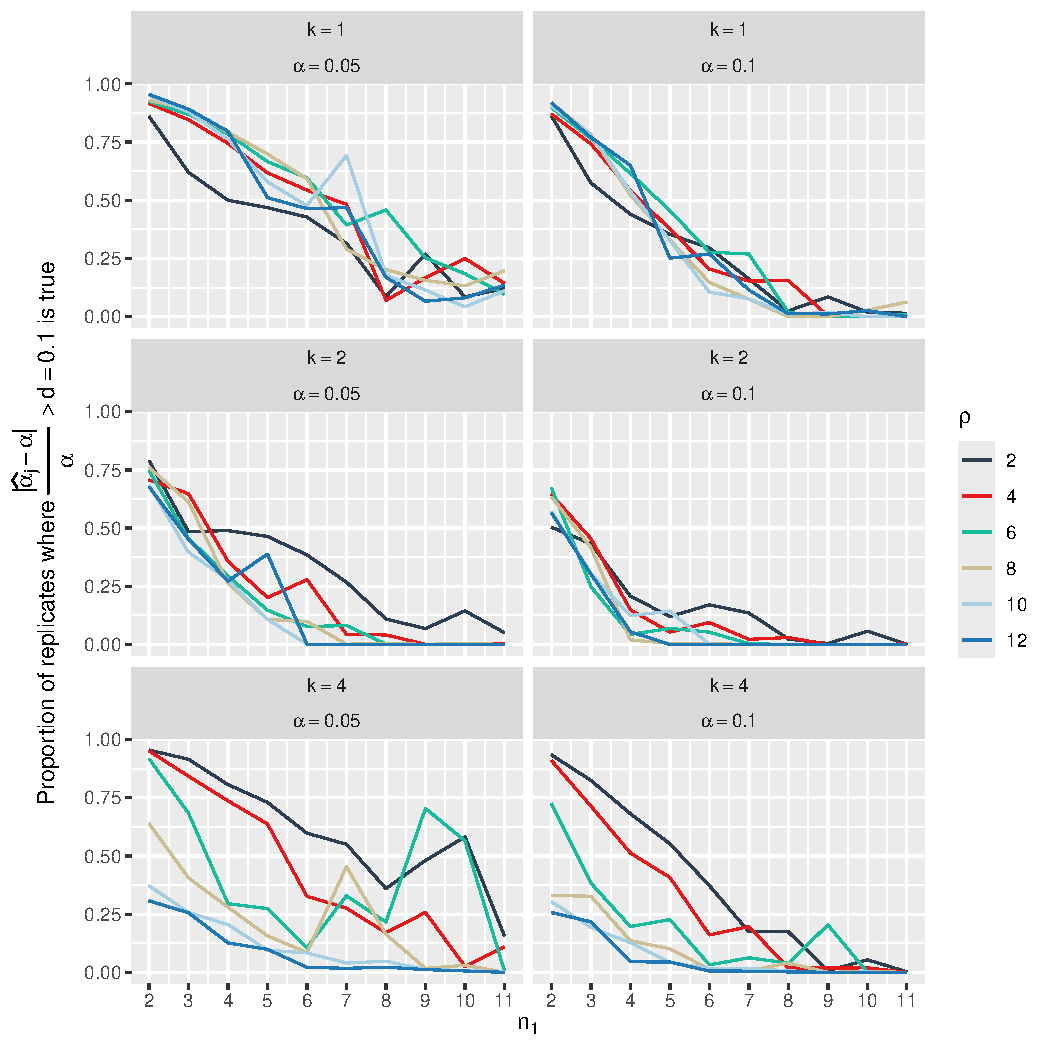
\includegraphics{some_simple_approaches_to_improve_the_Welch-Satterthwaite_approximation_files/figure-pdf/fig-sim-pro-rel-alpha-1.pdf}

}

\caption{\label{fig-sim-pro-rel-alpha}Graphical representation of
Table~\ref{tbl-sim-pro-rel-alpha}}

\end{figure}%

\section{Conclusion}\label{sec-conc}

\section{Appendix}\label{appendix}

\subsection{Degrees of freedom estimated by the WS
approach}\label{sec-df-ws}

In our case, following \citet{satterthwaite_approximate_1946} and
\citet{welch_generalization_1947}, the degrees of freedom
\(\widehat{\nu}\) can be expressed as:

\begin{equation}\phantomsection\label{eq-df-ws}{\begin{split}
  \widehat{\nu} & = \frac{\left( \frac{\widehat{\sigma}^2_1}{n_1} + \frac{\widehat{\sigma}^2_2}{n_2} \right)^2}{\frac{1}{n_1-1} \left( \frac{\widehat{\sigma}^2_1}{n_1} \right)^2 + \frac{1}{n_2-1} \left( \frac{\widehat{\sigma}^2_2}{n_2} \right)^2} \\
  & = \frac{\left( \frac{\widehat{\sigma}^2_1}{n_1} + \frac{\rho\widehat{\sigma}^2_1}{kn_1} \right)^2}{\frac{1}{n_1-1} \left( \frac{\widehat{\sigma}^2_1}{n_1} \right)^2 + \frac{1}{kn_1-1} \left( \frac{\rho\widehat{\sigma}^2_1}{kn_1} \right)^2} \\
  & = \frac{(n_1-1)(kn_1-1)(k+\rho)^2}{(kn_1-1)k^2 + (n_1-1)\rho^2}
  \end{split}}\end{equation}

\phantomsection\label{supplementary-material}
\bigskip

\begin{center}

{\large\bf SUPPLEMENTARY MATERIAL}

\end{center}

\begin{description}
\item[001\_simulation\_script.R]
R script used to produce the simulation results presented in
Table~\ref{tbl-sim-pro-rel-alpha} and Figure~\ref{fig-sim-pro-rel-alpha}
\item[simulation\_tbl\_stacked.csv]
Simulated dataset Table~\ref{tbl-sim-pro-rel-alpha}
\end{description}


\renewcommand\refname{References}
  \bibliography{bibliography.bib}


\end{document}
